\chapter{Коммутирующие наблюдаемые, энергетические фазы и прецессия спина}

\lectureoverview{Мы начинаем с качественного смысла неопределённости. Две наблюдаемые могут одновременно иметь определённые значения только тогда, когда у них есть полный общий собственный базис, и это эквивалентно коммутированию их операторов. Затем мы рассматриваем унитарную эволюцию и уравнение Schr\"odinger, сравниваем коммутаторы с классическими скобками Пуассона, решаем зависящее от времени уравнение в энергетическом базисе и применяем результат к спину в магнитном поле. Окончательный расчёт даёт прецессию средних значений спина, два энергетических уровня общего гамильтониана спина и различие между поперечным средним значением и фотоном с энергией, равной половине энергетического зазора.}

Спин с двумя состояниями остаётся нашей простейшей квантовой системой. Гильбертово пространство с тремя состояниями было бы следующей по простоте абстрактной возможностью; два спина уже имеют четыре ортогональных базисных состояния. Мы пока не будем составлять систему из двух спинов, хотя этот шаг уже близок и вместе с ним появится запутанность. Сначала следует завершить задачу об одном спине и прочнее обосновать идеи неопределённости и временной эволюции.

\section{Когда две величины могут быть определёнными одновременно}

Хорошее измерение воспроизводимо. Если измеряется наблюдаемая и получено значение \(l\), то немедленное повторение должно дать то же значение. Следовательно, первое измерение должно оставить систему, по крайней мере на мгновение, в собственном состоянии соответствующего оператора:
\begin{equation}
L\ket{l}=l\ket{l}.
\end{equation}
Этого операционального утверждения достаточно, чтобы выявить качественное происхождение неопределённости.

Предположим, что две наблюдаемые \(L\) и \(M\) можно измерить одновременно. Совместное измерение должно оставлять определёнными оба сообщённых значения. Поэтому его возможные постизмерительные состояния должны быть одновременными собственными векторами обоих операторов. В рассматриваемом здесь конечномерном случае мы можем выбрать полный ортонормированный набор \(\{\ket{i}\}\), удовлетворяющий
\begin{equation}
L\ket{i}=l_i\ket{i},
\qquad
M\ket{i}=m_i\ket{i}.
\label{eq:l5-common-eigenvectors}
\end{equation}

\begin{remark}
Слово \emph{базис} будет означать полный ортонормированный базис. Линейная алгебра допускает неортогональные базисы, но для квантовых состояний соглашение об ортонормированности особенно естественно. Вырожденные собственные значения оставляют свободу внутри собственного подпространства; в этом пространстве собственные векторы можно выбрать ортонормированными.
\end{remark}

\begin{theorem}
Две эрмитовы наблюдаемые в конечномерном пространстве можно измерять одновременно тогда и только тогда, когда они допускают полный общий собственный базис; эквивалентно, когда они коммутируют.
\end{theorem}

Прямое направление сразу следует из уравнения~\eqref{eq:l5-common-eigenvectors}. При действии в одном порядке получаем
\begin{align}
ML\ket{i}
&=M\bigl(l_i\ket{i}\bigr)\\
&=l_i m_i\ket{i},
\end{align}
а в обратном порядке получаем
\begin{align}
LM\ket{i}
&=L\bigl(m_i\ket{i}\bigr)\\
&=m_i l_i\ket{i}.
\end{align}
Собственные значения — обычные числа, поэтому \(l_i m_i=m_i l_i\). Следовательно, \(ML\) и \(LM\) действуют одинаково на каждом векторе базиса, а значит, и на любом состоянии:
\begin{equation}
[L,M]\equiv LM-ML=0.
\label{eq:l5-commuting-condition}
\end{equation}

\begin{figure}[htbp]
\centering
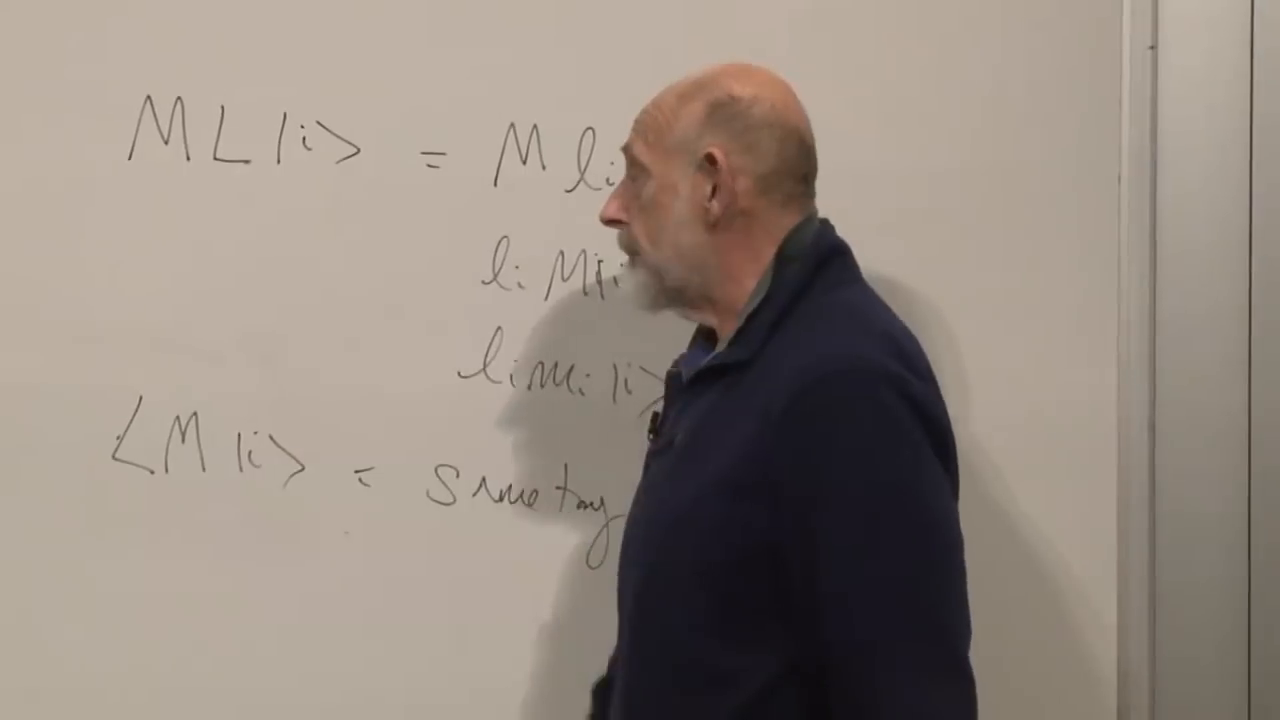
\includegraphics[width=0.86\textwidth]{lecture_05_figure_02.png}
\caption{Аргумент с общими собственными векторами приводит к \(LM-ML=[L,M]=0\).}
\lectureframe{00:10:30}
\end{figure}

Верно и обратное: коммутирующие эрмитовы операторы можно одновременно диагонализовать. Если у одного оператора есть вырожденное собственное подпространство, то другой сохраняет это подпространство, и внутри него его можно диагонализовать. Повторяя это в каждом собственном подпространстве, получаем полный общий собственный базис.

Операторы Паули дают первый важный контрпример. Никакие два из \(\sigma_x,\sigma_y,\sigma_z\) не коммутируют. Собственные состояния \(\sigma_z\) — это вверх и вниз, а собственные состояния \(\sigma_x\) — вправо и влево. Можно приготовить любую из компонент резко определённой и повторять её измерение, но нельзя сразу приготовить обе компоненты резко определёнными. Это и есть неопределённость ещё до введения какого-либо численного неравенства.

Позже мы количественно опишем, как неопределённости двух некоммутирующих наблюдаемых ограничивают друг друга. Здесь не доказывается никакой численный принцип неопределённости. Существо нынешнего утверждения предшествует неравенству: некоммутативность не позволяет состоянию приписывать обеим величинам одновременно определённые значения.

\begin{classroomqa}
\audiencequestion{Почему совместное измерение требует общих собственных векторов?}
\lecturerresponse{Воспроизводимое измерение оставляет состояние, в котором измеренное значение определено, а это означает собственное состояние измеряемого оператора. Если два значения получены вместе и оба остаются воспроизводимыми, то результирующее состояние должно быть собственным состоянием обоих операторов. Поэтому полный набор совместных исходов образует общий собственный базис.}
\end{classroomqa}

\begin{classroomqa}
\audiencequestion{Требует ли это двух разных частиц?}
\lecturerresponse{Не обязательно, поскольку \(\sigma_x\) и \(\sigma_z\) уже действуют на один спин. Однако для двух различных подсистем наблюдаемые, действующие на разных множителях, действительно коммутируют: \(A\otimes I\) коммутирует с \(I\otimes B\). Именно поэтому компоненту одного спина и компоненту другого можно измерить совместно. Объединение таких систем позже приведёт к запутанности.}
\end{classroomqa}

\section{Унитарная эволюция и её генератор}

Квантовой механике понадобилось значительно больше времени, чем классической механике, чтобы определить, что такое состояние, но как только пространство состояний установлено, правило движения записывается компактно. Пусть
\begin{equation}
\ket{\psi(t)}=U(t)\ket{\psi(0)}.
\label{eq:l5-propagator}
\end{equation}
Временная эволюция должна сохранять различимость состояний. Более того, она сохраняет все скалярные произведения. Для ортонормированного базиса,
\begin{equation}
\bra{j}U^\dagger(t)U(t)\ket{i}=\delta_{ji},
\end{equation}
и потому
\begin{equation}
U^\dagger(t)U(t)=I.
\label{eq:l5-unitarity}
\end{equation}
Оператор эволюции унитарен.

При нулевом промежутке времени \(U(0)=I\). Тогда непрерывность означает, что эволюция за малое время \(\epsilon\) лишь слегка отличается от тождественного оператора. В единицах, где \(\hbar=1\), запишем
\begin{equation}
U(\epsilon)=I-i\epsilon H+O(\epsilon^2),
\qquad
U^\dagger(\epsilon)=I+i\epsilon H^\dagger+O(\epsilon^2).
\end{equation}
Подстановка в уравнение~\eqref{eq:l5-unitarity} даёт
\begin{equation}
H^\dagger=H.
\end{equation}
Генератор временной эволюции эрмитов и потому является наблюдаемой. Это гамильтониан.

Применяя бесконечно малый пропагатор к состоянию, получаем
\begin{equation}
\ket{\psi(\epsilon)}
=\ket{\psi(0)}-i\epsilon H\ket{\psi(0)}+O(\epsilon^2).
\end{equation}
После перегруппировки получаем разностное отношение, написанное на доске:
\begin{equation}
\frac{\ket{\psi(\epsilon)}-\ket{\psi(0)}}{\epsilon}
=-iH\ket{\psi(0)}+O(\epsilon).
\end{equation}

\begin{figure}[htbp]
\centering
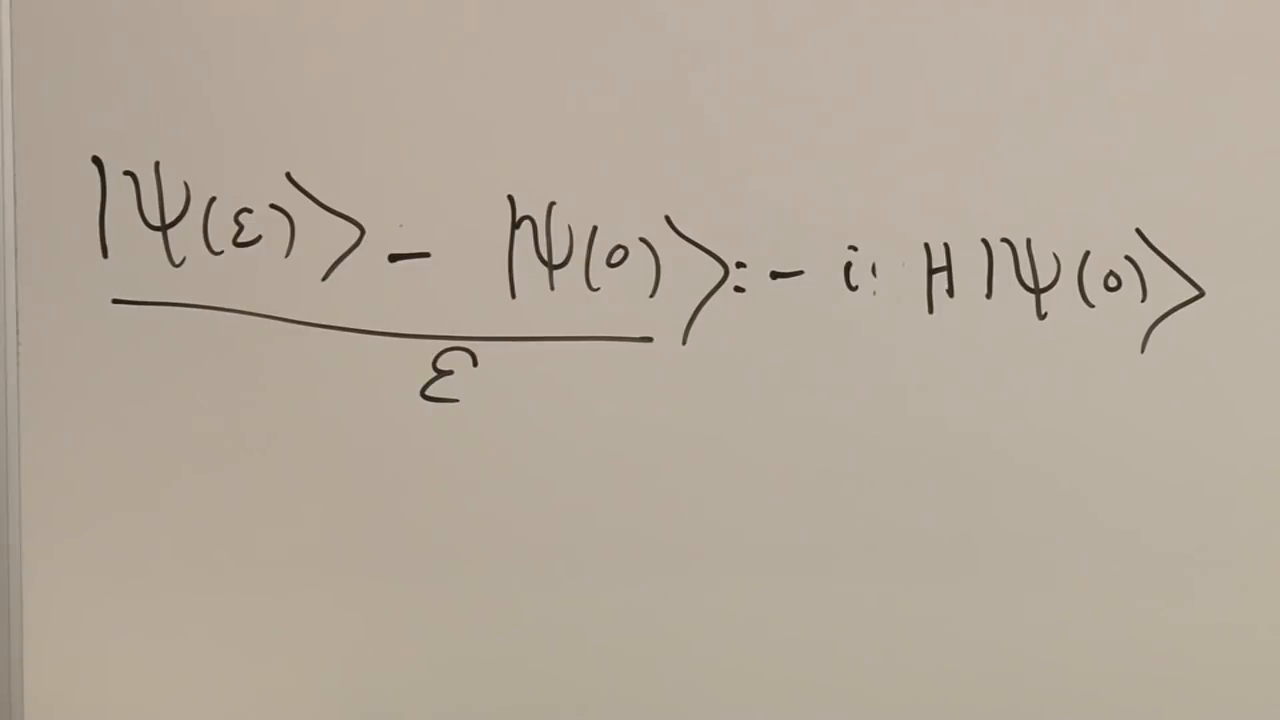
\includegraphics[width=0.86\textwidth]{lecture_05_figure_03.png}
\caption{Бесконечно малое приращение, записанное в виде разностного отношения.}
\lectureframe{00:23:33}
\end{figure}

Переход \(\epsilon\to0\) даёт зависящее от времени уравнение Schr\"odinger:
\begin{equation}
\frac{d}{dt}\ket{\psi(t)}=-iH\ket{\psi(t)}.
\label{eq:l5-schrodinger}
\end{equation}
При восстановлении констант это \(i\hbar\,d\ket{\psi}/dt=H\ket{\psi}\).

Исходное уравнение Schr\"odinger относилось к волновой функции движущейся частицы. Приведённое выше операторное соотношение когда-то называли обобщённым уравнением Schr\"odinger, потому что оно в равной мере применимо к спину, системе с тремя состояниями, двум спинам или системе сколь угодно большой сложности. Это прилагательное по большей части вышло из употребления; теперь это просто общая форма уравнения.

Уравнение~\eqref{eq:l5-schrodinger} задаёт определённую эволюцию состояния, когда система остаётся невозмущённой. Это не делает определённым каждый экспериментальный исход. Квантовое состояние задаёт вероятности возможных измерений, а уравнение обновляет эти вероятности через изменяющиеся амплитуды. Измерение, как правило, изменяет состояние и прерывает эту изолированную эволюцию.

\begin{classroomqa}
\audiencequestion{Всякое ли измерение возмущает систему?}
\lecturerresponse{Вообще говоря, да, но есть важный частный случай. Если состояние уже является собственным состоянием наблюдаемой, то идеальное воспроизводимое измерение может подтвердить её значение, не изменяя это состояние. В общем случае невозможна именно возможность измерить произвольную наблюдаемую, не возмутив другие, несовместимые свойства.}
\end{classroomqa}

\section{Энергия и не зависящее от времени уравнение}

Поскольку \(H\) эрмитов, его собственные значения вещественны, а его собственные векторы можно выбрать в виде полного ортонормированного базиса:
\begin{equation}
H\ket{E_i}=E_i\ket{E_i}.
\label{eq:l5-time-independent}
\end{equation}
Это не зависящая от времени форма уравнения Schr\"odinger. Это задача на собственные значения, а не уравнение движения: она спрашивает, какие значения энергии может иметь система и в каких состояниях эти значения определены резко.

Спектр зависит от системы. Связанное движение в атоме и гармонический осциллятор имеют счётные уровни энергии. Несвязанная частица может иметь непрерывный спектр. Энергию можно измерять многими способами; в принципе даже достаточно точное измерение массы могло бы использовать \(E=mc^2\), хотя на практике это редко бывает рабочим методом. У реальной системы уже есть свой гамильтониан; физик не предписывает его, а пытается обнаружить. Как только этот оператор известен, математической задачей становится нахождение его собственных значений и собственных векторов.

Добавление константы \(cI\) к \(H\) сдвигает каждую энергию на \(c\). Это умножает всё состояние на одну общую фазу \(e^{-ict}\), которая не меняет вероятностей или средних значений. На рассматриваемую здесь динамику влияют только разности энергий.

\section{Как изменяются средние значения}

Стандартный термин \emph{среднее значение} означает статистическое среднее. Для наблюдаемой \(L\),
\begin{equation}
\expect{L}(t)=\bra{\psi(t)}L\ket{\psi(t)}.
\end{equation}
На этом этапе временная зависимость содержится только во векторах состояния. Дифференцируя обе части и используя уравнение~\eqref{eq:l5-schrodinger} вместе с его эрмитово-сопряжённым,
\begin{equation}
\frac{d}{dt}\ket{\psi}=-iH\ket{\psi},
\qquad
\frac{d}{dt}\bra{\psi}=i\bra{\psi}H,
\end{equation}
получаем
\begin{align}
\frac{d}{dt}\expect{L}
&=i\bra{\psi}HL\ket{\psi}
  -i\bra{\psi}LH\ket{\psi}\\
&=-i\expect{[L,H]}.
\label{eq:l5-expectation-motion}
\end{align}

\begin{figure}[htbp]
\centering
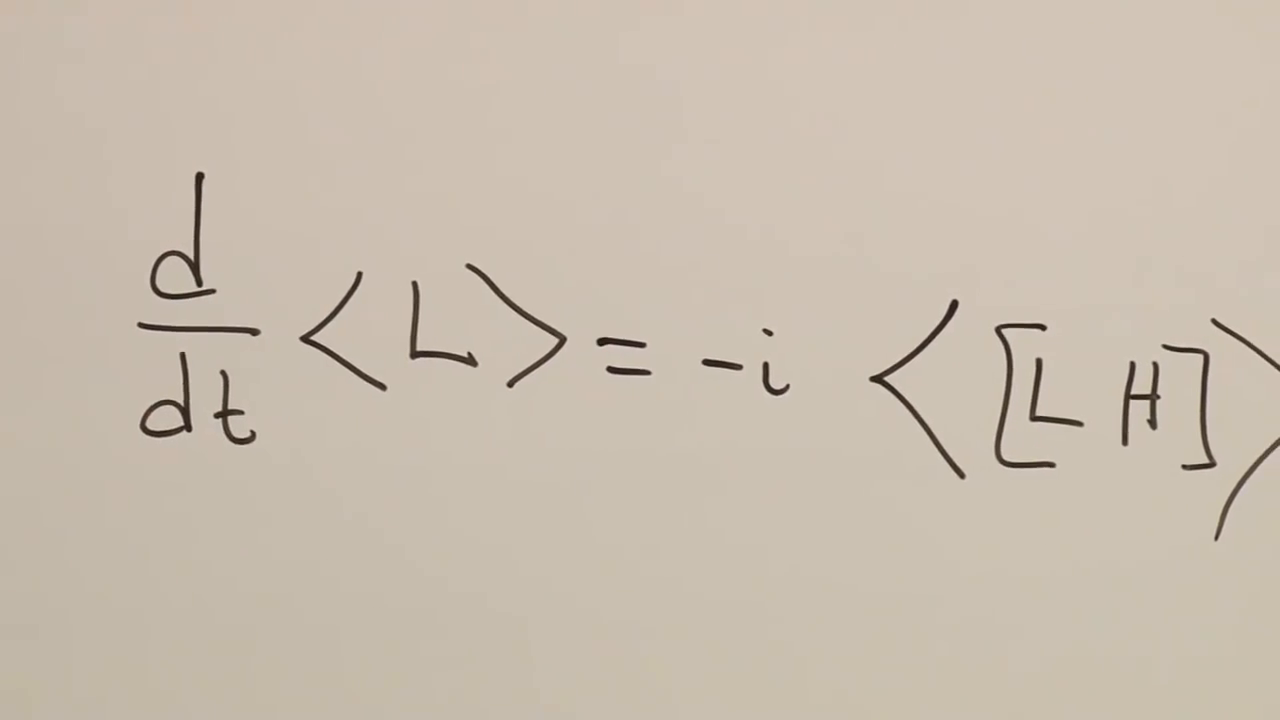
\includegraphics[width=0.86\textwidth]{lecture_05_figure_04.png}
\caption{Уравнение движения для среднего значения в коммутаторной форме.}
\lectureframe{00:35:35}
\end{figure}

Множитель \(i\) не ставит под угрозу вещественность \(\expect{L}\). Для эрмитовых \(L\) и \(H\) коммутатор антиэрмитов:
\begin{equation}
[L,H]^\dagger=-[L,H].
\end{equation}
Поэтому его среднее значение чисто мнимо, так что умножение на \(-i\) дает вещественную производную.

Иногда пишут сокращенно
\begin{equation}
\dot L=-i[L,H].
\end{equation}
На данном этапе это следует читать как сокращение для уравнения~\eqref{eq:l5-expectation-motion}, то есть уравнения о средних значениях. Полная смена представления, при которой временную зависимость несут сами операторы, будет рассмотрена позже.

\subsection{Алгебра коммутаторов}

Коммутаторы антисимметричны:
\begin{equation}
[A,B]=-[B,A].
\end{equation}
Они также подчиняются правилу произведения, аналогичному правилу Лейбница для производных:
\begin{equation}
[AB,C]=A[B,C]+[A,C]B.
\label{eq:l5-product-rule}
\end{equation}
Чтобы это проверить, сохраняйте порядок каждого множителя:
\begin{align}
A[B,C]+[A,C]B
&=A(BC-CB)\\
&\quad +(AC-CA)B\\
&=ABC-ACB\\
&\quad +ACB-CAB\\
&=ABC-CAB\\
&=[AB,C].
\end{align}

\begin{figure}[htbp]
\centering
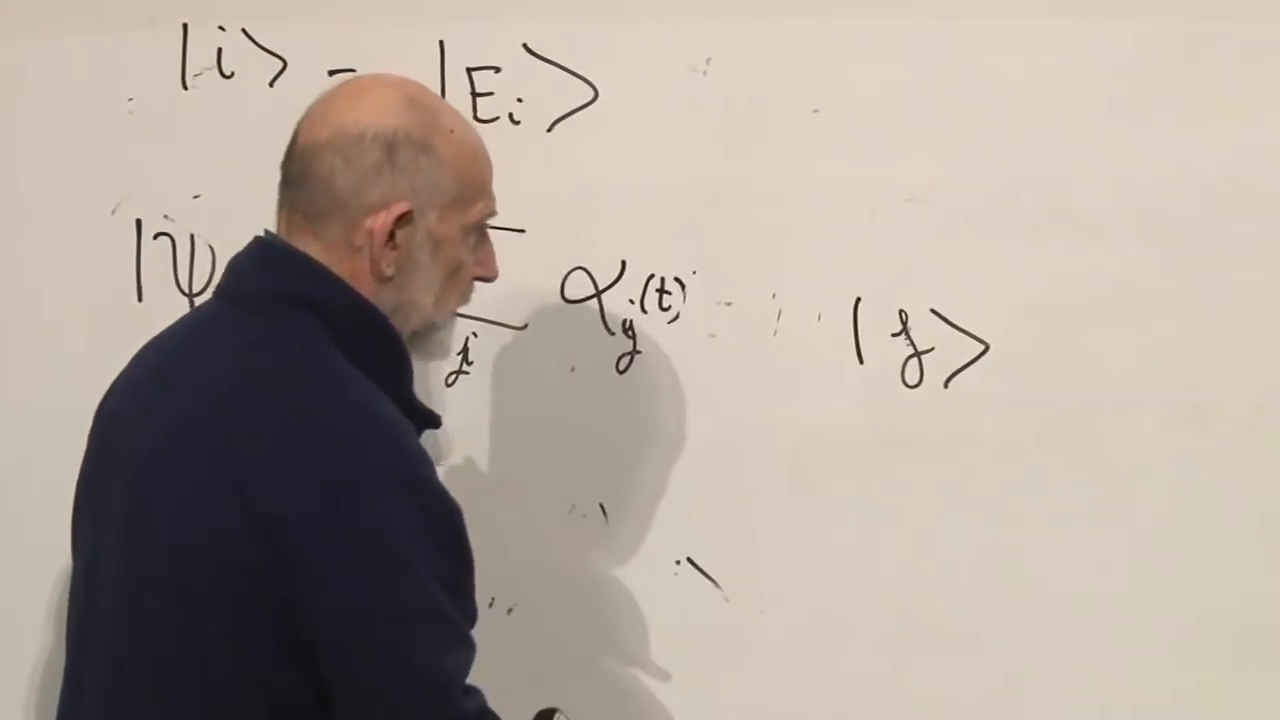
\includegraphics[width=0.86\textwidth]{lecture_05_figure_05.png}
\caption{Проверка правила произведения для коммутатора путем разложения обеих частей.}
\lectureframe{00:43:10}
\end{figure}

\begin{classroomqa}
\audiencequestion{Не учитывает ли правая часть правила произведения левую случайно дважды?}
\lecturerresponse{Нет. После раскрытия скобок \(ABC\) и \(-CAB\) — это два нужных члена. Два вставленных члена — \(-ACB\) и \(+ACB\), и они точно сокращаются. Кажущаяся лишняя копия — это временный член, необходимый, чтобы разложить выражение на множители двумя требуемыми способами.}
\end{classroomqa}

Та же антисимметрия и то же правило произведения выполняются для классических скобок Пуассона. Это структурное сходство не случайно. Классическое соответствие имеет вид
\begin{equation}
\{A,B\}
\quad\longleftrightarrow\quad
\frac{1}{i\hbar}[A,B]
=-\frac{i}{\hbar}[A,B].
\label{eq:l5-poisson-correspondence}
\end{equation}
В единицах \(\hbar=1\) классическое уравнение
\begin{equation}
\frac{dL}{dt}=\{L,H\}
\end{equation}
имеет тот же вид, что и уравнение~\eqref{eq:l5-expectation-motion}. В обычных макроскопических единицах \(\hbar\) очень мало, и в соответствующем классическом пределе коммутаторы становятся пренебрежимо малыми. Это существенная проверка, которая отождествляет квантовый генератор \(H\) с гамильтонианом классической механики.

Множитель \(\hbar\) необходим по соображениям размерности. Скобка Пуассона включает дифференцирование по сопряженным координатам и импульсам, тогда как операторный коммутатор строится непосредственно из произведений. Постоянная Планка обеспечивает перевод между этими размерностями.

Положим \(L=H\). Поскольку всякий оператор коммутирует сам с собой,
\begin{equation}
\frac{d}{dt}\expect{H}
=-i\expect{[H,H]}=0.
\end{equation}
Для обсуждаемых не зависящих от времени гамильтонианов средняя энергия сохраняется. Возможно и более сильное утверждение о полном распределении энергии, но здесь требуется только среднее значение.

\begin{classroomqa}
\audiencequestion{Что означает \(L\) в этих уравнениях? Это момент импульса?}
\lecturerresponse{Здесь \(L\) — произвольный эрмитов линейный оператор, то есть любая наблюдаемая величина. Это может быть компонента спина, координата или даже сам \(H\). Буква выбрана от \emph{линейный оператор} и не должна пониматься как момент импульса, если только этот смысл не оговорен отдельно.}
\end{classroomqa}

\begin{classroomqa}
\audiencequestion{Почему множитель \(i\) не приводит к тому, что у вещественного среднего появляется мнимая производная?}
\lecturerresponse{Коммутатор двух эрмитовых операторов антиэрмитов, поэтому его среднее значение мнимо. Приведенное ниже вычисление с матрицами Паули делает это наглядным: их коммутаторы содержат явный множитель \(2i\), который сокращает \(-i\) в уравнении движения.}
\end{classroomqa}

\section{Решение уравнения Schr\"odinger в энергетическом базисе}

Предположим, что задача на собственные значения энергии решена. Разложим произвольное состояние по фиксированному энергетическому базису:
\begin{equation}
\ket{\psi(t)}=\sum_j\alpha_j(t)\ket{E_j}.
\label{eq:l5-energy-expansion}
\end{equation}
Векторы базиса в этом описании не меняются; вся временная зависимость заключена в коэффициентах. Подстановка уравнения~\eqref{eq:l5-energy-expansion} в уравнение~\eqref{eq:l5-schrodinger} дает
\begin{align}
\sum_j\dot\alpha_j(t)\ket{E_j}
&=-i\sum_j\alpha_j(t)H\ket{E_j}\\
&=-i\sum_j E_j\alpha_j(t)\ket{E_j}.
\end{align}
Единственность разложения по базису означает, что для каждого фиксированного \(j\)
\begin{equation}
\dot\alpha_j(t)=-iE_j\alpha_j(t),
\qquad\text{no sum on \(j\)}.
\end{equation}
Решение имеет вид
\begin{equation}
\alpha_j(t)=\alpha_j(0)e^{-iE_jt}.
\label{eq:l5-energy-phase}
\end{equation}

\begin{figure}[htbp]
\centering
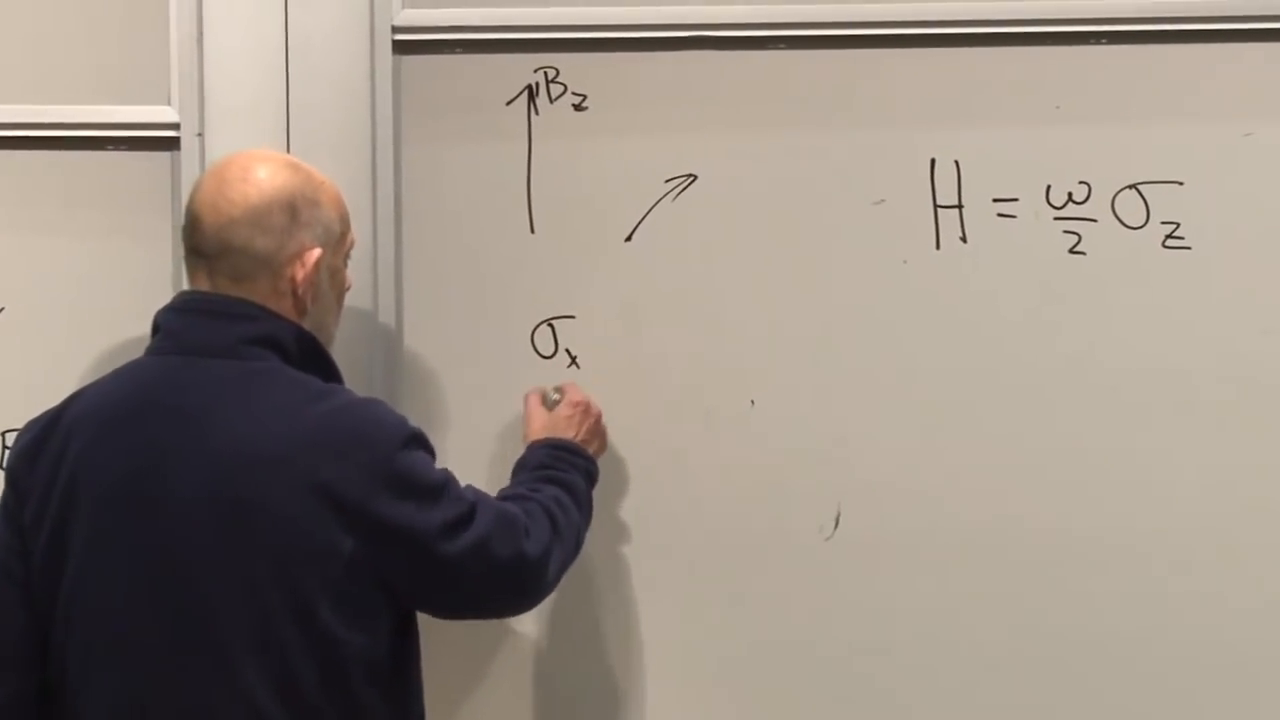
\includegraphics[width=0.86\textwidth]{lecture_05_figure_06.png}
\caption{Каждый коэффициент энергетического базиса удовлетворяет собственному уравнению с экспоненциальной фазой.}
\lectureframe{01:03:25}
\end{figure}

Таким образом, общее решение имеет вид
\begin{equation}
\ket{\psi(t)}
=\sum_j\alpha_j(0)e^{-iE_jt}\ket{E_j}.
\label{eq:l5-general-solution}
\end{equation}
Восстановление размерных единиц заменяет \(E_jt\) на \(E_jt/\hbar\). Модуль каждого коэффициента остается неизменным:
\begin{equation}
|\alpha_j(t)|=|\alpha_j(0)|.
\end{equation}
Временная эволюция изменяет относительные фазы. Отдельное собственное состояние энергии приобретает только одну общую фазу и поэтому имеет не зависящие от времени вероятности измерения.

Среднее значение \(L\) теперь можно записать явно. Определим его матричные элементы в энергетическом базисе как
\begin{equation}
L_{kj}=\bra{E_k}L\ket{E_j}.
\end{equation}
Тогда
\begin{align}
\expect{L}(t)
&=\sum_{k,j}
\alpha_k^*(0)\alpha_j(0)
e^{i(E_k-E_j)t}
L_{kj}.
\label{eq:l5-heisenberg-matrix}
\end{align}

\begin{figure}[htbp]
\centering
\includegraphics[width=0.86\textwidth]{lecture_05_figure_07.png}
\caption{Матричная формула в энергетическом базисе: каждый элемент несет фазовый множитель с частотой перехода.}
\lectureframe{01:10:45}
\end{figure}

Диагональные члены \(k=j\) постоянны. Внедиагональный матричный элемент осциллирует с энергетической разностью \(E_k-E_j\). В принятом здесь историческом изложении Heisenberg распознал эту матричную структуру еще до появления современного вывода через векторы состояния; обозначения Dirac позже сделали ее смысл прозрачным.

\begin{classroomqa}
\audiencequestion{Остаются ли модули коэффициентов \(\alpha_j\) неизменными?}
\lecturerresponse{Да. Каждый коэффициент умножается на комплексную фазу единичного модуля. Меняются только относительные фазы, и именно они позволяют средним значениям, содержащим внедиагональные матричные элементы, меняться со временем.}
\end{classroomqa}

\begin{classroomqa}
\audiencequestion{Должна ли в уравнении Schr\"odinger стоять частная производная или полная?}
\lecturerresponse{Для абстрактного состояния \(\ket{\psi(t)}\), используемого здесь, время — единственная явно указанная переменная, так что обе записи выражают одно и то же. Позже волновая функция, такая как \(\psi(x,t)\), будет зависеть и от координаты, и от времени, и тогда обозначение частной производной станет естественным.}
\end{classroomqa}

\begin{classroomqa}
\audiencequestion{Является ли сохранение ортогональности всего лишь эмпирическим предположением?}
\lecturerresponse{Оно подтверждается экспериментом, но также обладает необычной жесткостью. Попытки деформировать унитарную квантовую механику, как правило, разрушают положительность или сохранение вероятности, причинную локальность либо согласованное описание составных систем. David Finkelstein описывал деформируемые теории как испытывающие пластическое течение, а жесткие — как хрупкое растрескивание. Квантовая механика в этом смысле хрупка: малые произвольные изменения обычно не оставляют рядом согласованной теории.}
\end{classroomqa}

\begin{classroomqa}
\audiencequestion{Почему собственные значения энергии \(E_j\) вещественны?}
\lecturerresponse{Унитарность влечет, что бесконечно малый генератор \(H\) эрмитов, а всякое собственное значение эрмитова оператора вещественно. Следовательно, цепочка такова: сохранение ортогональности, унитарность, эрмитовость \(H\) и вещественность энергетического спектра.}
\end{classroomqa}

\section{Спин в магнитном поле}

Какой гамильтониан следует приписать одному спину? Изолированный спин в остальном пустом пространстве не имеет никакого нетривиального выделенного направления, поэтому его гамильтониан пропорционален единичному оператору и не порождает никакой наблюдаемой динамики. Магнитное поле задает и энергию взаимодействия, и ось.

Пусть поле направлено вдоль \(z\). Заряженная частица со спином имеет магнитный момент, и знакомая энергия диполя пропорциональна ориентации этого момента относительно поля. Поглотим напряженность поля, магнитный момент, соглашение о знаке и \(\hbar\) в одну константу \(\omega\):
\begin{equation}
H=\frac{\omega}{2}\sigma_z.
\label{eq:l5-z-hamiltonian}
\end{equation}
Множитель \(1/2\) удобен, потому что коммутаторы Паули содержат множитель \(2\).

Классическую картину со стрелкой нужно использовать осторожно. Квантовый спин не обладает одновременно определенными компонентами \(x\), \(y\) и \(z\), так что никакая обычная стрелка не может сразу представить все его свойства. Полезным трехмерным объектом будет вектор средних значений, а не сам двухкомпонентный вектор состояния.

\subsection{Коммутаторы Паули}

Используем матричные представления
\begin{equation}
\begin{aligned}
\sigma_x&=
\begin{pmatrix}0&1\\1&0\end{pmatrix},\\[0.4em]
\sigma_y&=
\begin{pmatrix}0&-i\\i&0\end{pmatrix},\\[0.4em]
\sigma_z&=
\begin{pmatrix}1&0\\0&-1\end{pmatrix}.
\end{aligned}
\end{equation}
Например,
\begin{align}
[\sigma_z,\sigma_x]
&=
\begin{pmatrix}1&0\\0&-1\end{pmatrix}
\begin{pmatrix}0&1\\1&0\end{pmatrix}
-
\begin{pmatrix}0&1\\1&0\end{pmatrix}
\begin{pmatrix}1&0\\0&-1\end{pmatrix}\\
&=
\begin{pmatrix}0&1\\-1&0\end{pmatrix}
-
\begin{pmatrix}0&-1\\1&0\end{pmatrix}\\
&=2
\begin{pmatrix}0&1\\-1&0\end{pmatrix}
=2i\sigma_y.
\end{align}
Циклические соотношения имеют вид
\begin{equation}
\begin{aligned}
[\sigma_z,\sigma_x]&=2i\sigma_y,\\
[\sigma_x,\sigma_y]&=2i\sigma_z,\\
[\sigma_y,\sigma_z]&=2i\sigma_x.
\end{aligned}
\label{eq:l5-pauli-commutators}
\end{equation}
Если поменять местами любой из операндов, знак меняется на противоположный.

\begin{figure}[htbp]
\centering
\includegraphics[width=0.86\textwidth]{lecture_05_figure_08.png}
\caption{Три коммутатора Паули циклически замыкаются на сами матрицы Паули.}
\lectureframe{01:33:30}
\end{figure}

Эти соотношения имеют ту же циклическую структуру, что и классические скобки Пуассона для момента импульса. Они также замыкаются на тех же трех операторах, что делает уравнения движения особенно простыми.

\begin{classroomqa}
\audiencequestion{Нужно ли вычислять коммутаторы с помощью скобок бра-кет?}
\lecturerresponse{Нет. Умножение операторов представляется умножением матриц, поэтому матрицы \(2\times2\) дают удобное прямое вычисление. Вместо этого можно последовательно подействовать операторами на базисные состояния со спином вверх и вниз и получить тот же результат.}
\end{classroomqa}

\subsection{Прецессия средних значений}

Применим уравнение~\eqref{eq:l5-expectation-motion} к гамильтониану из уравнения~\eqref{eq:l5-z-hamiltonian}:
\begin{align}
\frac{d}{dt}\expect{\sigma_x}
&=-i\frac{\omega}{2}\expect{[\sigma_x,\sigma_z]}
=-\omega\expect{\sigma_y},\\
\frac{d}{dt}\expect{\sigma_y}
&=-i\frac{\omega}{2}\expect{[\sigma_y,\sigma_z]}
=+\omega\expect{\sigma_x},\\
\frac{d}{dt}\expect{\sigma_z}
&=-i\frac{\omega}{2}\expect{[\sigma_z,\sigma_z]}
=0.
\label{eq:l5-spin-motion}
\end{align}

\begin{figure}[htbp]
\centering
\begin{minipage}[c]{0.62\textwidth}
\centering
\includegraphics[width=\textwidth]{lecture_05_figure_09.png}
\end{minipage}\hfill
\begin{minipage}[c]{0.31\textwidth}
\centering
\begin{tikzpicture}[scale=0.78,>=Latex]
  \draw[->,thick] (0,0) -- (0,3.0) node[above] {\(z\parallel\bm B\)};
  \draw[dashed] (0,1.8) ellipse (1.45 and 0.42);
  \draw[->,very thick] (0,0) -- (1.05,1.8)
    node[right] {\(\expect{\bm\sigma}\)};
  \draw[->,thick] (1.38,1.67)
    arc[start angle=-12,end angle=245,x radius=1.45,y radius=0.42];
\end{tikzpicture}
\end{minipage}
\caption{Уравнения на доске и их геометрическое следствие: поперечные средние значения вращаются, тогда как компонента, параллельная полю, остаётся неизменной. Стрелка изображает три средних значения, а не скрытый классический спин.}
\lectureframe{01:35:28}
\end{figure}

Первые два уравнения описывают круговое движение в поперечной плоскости:
\begin{align}
\expect{\sigma_x}(t)
&=\expect{\sigma_x}(0)\cos\omega t
-\expect{\sigma_y}(0)\sin\omega t,\\
\expect{\sigma_y}(t)
&=\expect{\sigma_x}(0)\sin\omega t
+\expect{\sigma_y}(0)\cos\omega t.
\end{align}
Между тем \(\expect{\sigma_z}\) остаётся постоянным. Поэтому вектор средних значений прецессирует вокруг оси магнитного поля с угловой частотой \(\omega\).

В этом расчёте в представлении Schr\"odinger операторы являются фиксированными матрицами. Меняется состояние, и потому именно средние значения совершают знакомое гироскопическое движение.

\begin{classroomqa}
\audiencequestion{Как двумерное пространство состояний может приводить к трёхмерной картине прецессии?}
\lecturerresponse{Вектор состояния имеет две комплексные компоненты с точностью до нормировки и общей фазы. А изображаемый в реальном пространстве вектор — \(\bigl(\expect{\sigma_x},\expect{\sigma_y},\expect{\sigma_z}\bigr)\). Эти средние значения определяются состоянием и образуют представление вектора Блоха, но сами по себе вектором состояния не являются.}
\end{classroomqa}

\section{Наиболее общий гамильтониан одного спина}

Каждую эрмитову матрицу \(2\times2\) можно разложить как
\begin{equation}
H=aI+b_x\sigma_x+b_y\sigma_y+b_z\sigma_z,
\end{equation}
с вещественными коэффициентами. Слагаемое с единичной матрицей изменяет только общую фазу. Оставшиеся три коэффициента можно рассматривать как компоненты вектора. Обозначив его модуль через \(\omega/2\), а направление — единичным вектором \(\bm n\), получаем, что нетривиальный гамильтониан принимает вид
\begin{equation}
H=\frac{\omega}{2}\,\bm\sigma\cdot\bm n,
\qquad
\bm\sigma\cdot\bm n
=n_x\sigma_x+n_y\sigma_y+n_z\sigma_z.
\label{eq:l5-general-spin-h}
\end{equation}
Если \(\bm B=B\bm n\), то \(\bm n\) задаёт направление поля, тогда как \(\omega\) включает в себя его величину вместе с магнитным взаимодействием. Именно \(\bm n\), а не \(\omega\), фиксирует ориентацию.

Уравнение движения принимает компактный вид
\begin{equation}
\frac{d}{dt}\expect{\bm\sigma}
=\omega\,\bm n\times\expect{\bm\sigma}.
\end{equation}
Компонента вдоль \(\bm n\) коммутирует с \(H\) и остаётся постоянной; перпендикулярные компоненты прецессируют вокруг направления \(\bm n\).

\begin{classroomqa}
\audiencequestion{Почему гамильтониан имеет именно такой вид?}
\lecturerresponse{Существует только четыре линейно независимые эрмитовы матрицы \(2\times2\): \(I,\sigma_x,\sigma_y,\sigma_z\). Единичная матрица не даёт никакого наблюдаемого движения одного спина, поэтому любой нетривиальный не зависящий от времени гамильтониан одного спина есть вещественная линейная комбинация трёх матриц Паули. Магнитное поле объединяет эти три коэффициента в величину и направление.}
\end{classroomqa}

\begin{classroomqa}
\audiencequestion{Что именно представляет собой \(\omega\)?}
\lecturerresponse{Это скаляр, пропорциональный величине поля, умноженной на магнитный момент, причём обычные константы в него поглощены. Он задаёт как частоту прецессии, так и энергетическое расщепление. Единичный вектор \(\bm n\) задаёт направление поля.}
\end{classroomqa}

\subsection{Два энергетических уровня}

Записав уравнение~\eqref{eq:l5-general-spin-h} в матричном виде, получаем
\begin{equation}
\bm\sigma\cdot\bm n
=
\begin{pmatrix}
n_z & n_x-in_y\\
n_x+in_y & -n_z
\end{pmatrix}.
\end{equation}
Обозначим его собственные значения через \(\lambda_1,\lambda_2\). Его след равен нулю:
\begin{equation}
\lambda_1+\lambda_2=0.
\end{equation}
Для единичного вектора \(n_x^2+n_y^2+n_z^2=1\) его определитель равен
\begin{align}
\lambda_1\lambda_2
&=\det(\bm\sigma\cdot\bm n)\\
&=-n_z^2-(n_x-in_y)(n_x+in_y)\\
&=-(n_x^2+n_y^2+n_z^2)\\
&=-1.
\end{align}
Следовательно, два собственных значения равны
\begin{equation}
\lambda_\pm=\pm1.
\end{equation}

\begin{figure}[htbp]
\centering
\includegraphics[width=0.86\textwidth]{lecture_05_figure_10.png}
\caption{След и определитель определяют собственные значения \(\bm\sigma\cdot\bm n\): \(+1\) и \(-1\).}
\lectureframe{01:59:20}
\end{figure}

Следовательно,
\begin{equation}
E_\pm=\pm\frac{\omega}{2},
\qquad
\Delta E=E_+-E_-=\omega.
\label{eq:l5-spin-gap}
\end{equation}
Направление поля изменяет собственные векторы энергии, но не эти два собственных значения.

\begin{classroomqa}
\audiencequestion{Как испускание фотона связано с этими уровнями?}
\lecturerresponse{При учёте поля излучения более высокий спиновый уровень может перейти на нижний, испустив фотон энергии \(\Delta E=\omega\) в принятой здесь конвенции \(\hbar=1\). Тогда спин переходит из одной из двух противоположных ориентаций вдоль оси поля в другую. В расчёте прецессии это слабое радиационное взаимодействие опущено, поэтому до испускания спин может много раз прецессировать.}
\end{classroomqa}

\begin{classroomqa}
\audiencequestion{Почему магнитное поле рассматривается как число, а не как квантовый оператор?}
\lecturerresponse{Магнит пока рассматривается как тяжёлый классический прибор, флуктуациями и отдачей которого можно пренебречь. Полное описание включало бы его в более крупную квантовую систему. Такое практическое разделение на систему и прибор оправдано, когда у прибора много степеней свободы и его существенные переменные флуктуируют столь слабо, что электрон не может заметно их изменить.}
\end{classroomqa}

\begin{classroomqa}
\audiencequestion{Описывают ли гладкие уравнения прецессии каждое отдельное испытание?}
\lecturerresponse{Они описывают средние значения, а значит, усреднения по одинаково подготовленным испытаниям. Отдельные измерения остаются вероятностными. При многократных повторениях усреднение по выборке обычно приближается к теоретическому среднему, но теория вероятностей не гарантирует точного результата для каждой конечной последовательности, точно так же как миллион подбрасываний монеты не обязан дать ровно половину орлов.}
\end{classroomqa}

\begin{classroomqa}
\audiencequestion{Если спин направлен вбок, испускается ли при переходе половина фотона?}
\lecturerresponse{Нет. Состояние, в котором спин направлен вбок, является суперпозицией двух энергетических собственных состояний. В симметричном случае вероятность обнаружить его на верхнем уровне равна одной второй, и на нижнем — тоже одной второй. Поэтому оно может либо испустить один полный фотон энергии \(\omega\), либо не испустить ничего. Его средняя испущенная энергия может быть равна \(\omega/2\), но ни один отдельный фотон не несёт половины межуровневого расщепления.}
\end{classroomqa}

Теперь мы исчерпали всю нетривиальную не зависящую от времени динамику одного спина. Та же алгебра, которая впервые указала на неопределённость, порождает и его движение: некоммутирующие матрицы Паули приводят к тому, что гамильтониан вызывает прецессию, тогда как компонента, коммутирующая с ним, сохраняется. Следующее усложнение — не ещё один гамильтониан одного спина, а большее пространство состояний, в котором независимые системы можно объединять и запутывать.
